\begin{solution}{normal}
\definecolor{crimsonglory}{rgb}{0.75, 0.0, 0.2}
\textbf{\textcolor{crimsonglory}{Lemma.}} The molecular flux of molecules through the surface area $A$ of ice is given by 
\[\Phi = \frac{1}{4}n\left<v\right>.\]
\begin{proof}
Let $f(v)$ be the Maxwell-Boltzmann distribution of velocities of the particles. What this means is that the probability that a particle has velocity in $[v_x,v_x+dv_x]\times[v_y,v_y+dv_y]\times[v_z,v_z+dv_z]$ is
\[f\left(\sqrt{v_x^2+v_y^2+v_z^2}\right)dv_xdv_ydv_z.\]Set up spherical coordinates with origin at the hole. We will now count the number of particles that hit the hole in a time $dt$ using a funny double counting argument, where we start by counting the number of particles that hit the hole with a certain velocity and then integrate over all velocities.

We will start by counting the number of particles that move with speed $v$ (technically speed in $[v,v+dv]$, but from now on we'll be lazy about this) and spherical coordinate angles $(\theta,\phi)$. Here $\theta=0$ means pointing toward the hole, and $\theta=\pi/2$ is parallel to the plane of the hole (the spherical coordinates for the velocity are flipped compared to those for space, since the $\theta=0$ rays are anti-parallel). In a given volume $dV$, the number of particles with this velocity is just
\[(n dV)\cdot f(v)\cdot v^2\sin\theta \,dv \,d\theta\, d\phi.\]For this given velocity, the volume in space that will allow such particles to hit the hole is a tilted cone object with base $A$, slant $\theta$, slant height $vdt$, and aligned in the proper $\phi$ direction. In particular, its volume is $A(vdt)\cos\theta$, so the number of particles with velocity $(v,\theta,\phi)$ hitting the hole in time $dt$ is
\[(n A dt)\cdot f(v)\cdot v^3\sin\theta\cos\theta \,dv \,d\theta\, d\phi.\]Thus, the rate of particles leaving is
\[\alpha=n A\int_0^\infty v^3f(v)\,dv\int_0^{\pi/2}\sin\theta\cos\theta\,d\theta\int_0^{2\pi}d\phi=\pi n A\int_0^\infty v^3f(v)\,dv.\]Note that
\[\langle v\rangle=\int_0^\infty\int_0^\pi\int_0^{2\pi} v\cdot f(v)\cdot v^2\sin\theta\,dv\,d\theta\,d\phi=4\pi\int_0^\infty v^3f(v)\,dv,\]which tells us that
\[\alpha=\frac{n A}{4}\langle v\rangle,\]as desired. Note that proof didn't depend on the particular form of the Maxwell-Boltzmann speed distribution\footnote{Credits to \hyperlink{https://artofproblemsolving.com/community/c473124h1890945_diffusion_problem}{here} for the proof of this alternate thermodynamic system.} for the proof \footnote{Note that the flux here is only approximate as there will be an extra potential energy contribution to the vapors right after evaporation and since Maxwell's distribution is based on Boltzmann factors, we can't really calculate the extra energy that is added to the partition function. However, we can neglect these contributions as they are very small.}.
\end{proof}
This means that the mass flow rate of the molecules leaving the teacup is given by\footnote{This method is only approximate of the actual value of $L$ because some of the molecules that escape the teacup will actually go back. However, the number of molecules that bounce back is very slim so we can neglect them.} 
\[w = \frac{\rho_0 \left<v\right> A}{4}.\]
The time $t$ for the complete evaporation ice will then be given by 
\[t \approx \frac{m}{w} = \frac{4m}{\rho \left<v\right> A}\]
where $m$ is the mass of the ice in the teacup. As we are to estimate the dimensions of the cup ourselves, let us do just that. Most convential teacups hold up to $150\;\mathrm{mL}$ of water and since the density of ice is $0.91\;\mathrm{g/cm^3}$, we can estimate the mass of the ice in the water to be $m \approx 136\;\mathrm{g}$. The area of a cup of tea is $A \approx \pi (4.5)^2 \approx 63\;\mathrm{cm^3}$. 
\vspace{3mm}

\noindent Measurements were done with this teacup:
\begin{center}
    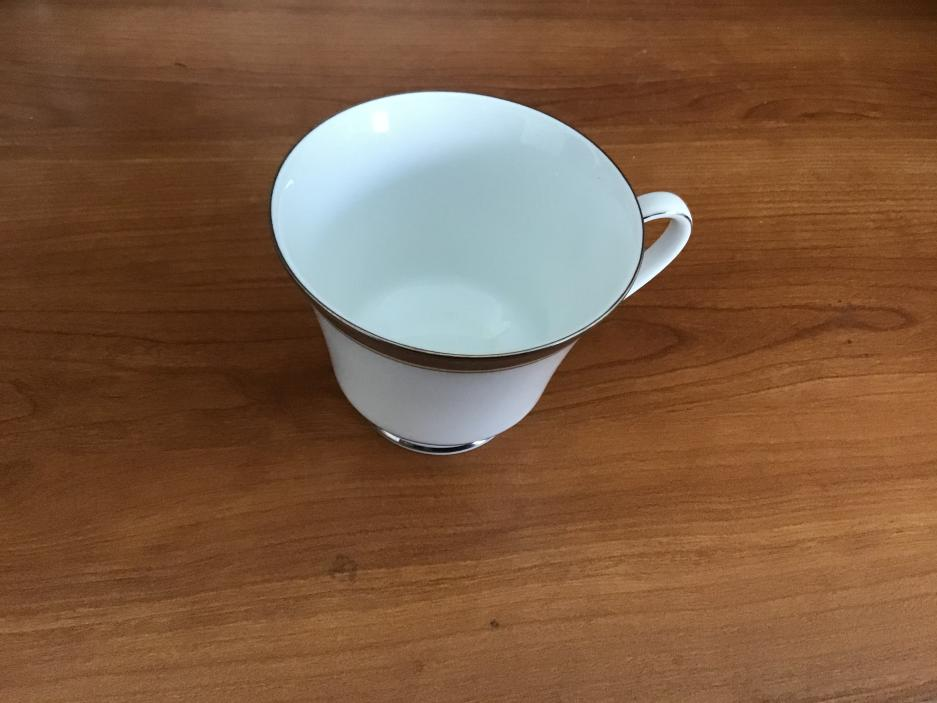
\includegraphics[width=10cm]{teacup.jpg}
\end{center}

The average velocity is given by 
\[\left<v\right> = \int_{0}^{\infty} v f(v)\text{d}v = \sqrt{\frac{8RT}{\pi \mu}}\]
which means that 
\[t = \frac{4m}{\rho \left<v\right> A} = \frac{4m}{\rho_0 A}\sqrt{\frac{\pi \mu}{8R T}} = \frac{m}{\rho_0 A}\sqrt{\frac{2\pi \mu}{RT}}.\]
By the ideal gas law, the vapor pressure can be represented as $\rho_0 = \frac{P\mu}{RT}$ which means that 
\[t = \frac{m}{\rho_0 A}\sqrt{\frac{2\pi \mu}{RT}} = \frac{mRT}{P\mu A}\sqrt{\frac{2\pi \mu}{RT}}= \frac{m}{PA}\sqrt{\frac{2\pi RT}{\mu}}.\]
While the ice is in motion, the astronaut experiences a force given from problem 21 which implies that the astronauts acceleration is (given that the astronauts mass is $M \approx 130\;\mathrm{kg}$):
\[F = \frac{PA}{2}\implies a = \frac{PA}{2M}\]
This means that 
\begin{align*}
L_{\text{acceleration}} = \frac{1}{2}at^2 &= \frac{1}{2}\left(\frac{PA}{2M}\right)\left(\frac{m}{PA}\sqrt{\frac{2\pi RT}{\mu}}\right)^2\\
&= \frac{1}{2}\left(\frac{PA}{2M}\right)\left(\frac{2\pi m^2 RT}{P^2 A^2 \mu}\right) \\
&= \frac{m^2}{2M}\frac{\pi RT}{PA\mu} \\
&= \frac{(0.136\;\mathrm{kg})^2}{2\cdot 130\;\mathrm{kg}}\frac{\pi \cdot 8.3\;\mathrm{J\cdot mol^{-1}\cdot K^{-1}}\cdot 272\;\mathrm{K}}{550\;\mathrm{Pa}\cdot 0.0063\;\mathrm{m^2}\cdot 0.018\;\mathrm{kg/mol}} \approx 88\;\mathrm{m}
\end{align*}
After the astronaut has stopped accelerating, it will be moving at a constant velocity of 
\[v = at = \left(\frac{PA}{2M}\right)\left(\frac{m}{PA}\sqrt{\frac{2\pi RT}{\mu}}\right) = \frac{m}{2M}\sqrt{\frac{2\pi RT}{\mu}} \approx 0.46\;\mathrm{m/s}.\]
The velocity is constant since after sublimation, there are no other external forces acting on the astronaut. Since this is happening in a vacuum, the astronaut could potentially move at a constant velocity until infinity. However, the aim of this problem is to estimate how realistic the method is. This means that we should aim to look at a realistic time that the astronaut travels the extra distance to the space station a distance of $L = 100\;\mathrm{m}$ away. The extra distance travelled will be 
\[L_{\text{velocity}} = v (\tau - t) = \left(\tau - \frac{m}{PA}\sqrt{\frac{2\pi RT}{\mu}}\right)\frac{m}{2M}\sqrt{\frac{2\pi RT}{\mu}}\]
where $\tau$ is the total time of travel. The total length travelled is then 
\[L = L_{\text{acceleration}} + L_{\text{velocity}} = \frac{m^2}{2M}\frac{\pi RT}{PA\mu} + \left(\tau - \frac{m}{PA}\sqrt{\frac{2\pi RT}{\mu}}\right)\frac{m}{2M}\sqrt{\frac{2\pi RT}{\mu}}.\]
We now solve for $\tau$. By substituting values, we yield
\[100 \approx 88 + 0.46(\tau - 35)\implies \tau \approx 252\;\mathrm{s}.\]
This is a realistic amount of time for the total travel, so yes, this method is realistic to use. 


\end{solution}